% Gabarit pandoc des corrigés publiés (brut et guidé). Contenu sans marque ni nom de site.
% Compilation : lualatex (latexmk -lualatex).
% Le Markdown reste la source unique : ne pas éditer ce fichier .tex à la main.
\documentclass[11pt,a4paper]{article}

% --- Moteur, polices (Latin Modern) et langue ---------------------------------
\usepackage{iftex}
\ifLuaTeX\else\errmessage{Ce document se compile avec lualatex}\fi
\usepackage{amsmath,amssymb,mathtools}
\usepackage{fontspec}
% mathrm=sym : \mathrm prend ses glyphes dans la police mathématique (ℓ, μ, Ω), comme KaTeX.
\usepackage[math-style=TeX,bold-style=TeX,mathrm=sym]{unicode-math}
% Repli pour les glyphes absents de Latin Modern (indices et exposants Unicode,
% flèches, filets des schémas en texte, symboles) : DejaVu, puis Latin Modern Math
% (ℓ, lettres mathématiques Unicode des légendes).
\directlua{
  luaotfload.add_fallback("repliTexte", {"DejaVuSerif:mode=harf;", "DejaVuSans:mode=harf;", "file:latinmodern-math.otf:mode=harf;"})
  luaotfload.add_fallback("repliMono", {"DejaVuSansMono:mode=harf;", "DejaVuSans:mode=harf;", "file:latinmodern-math.otf:mode=harf;"})
}
\setmainfont{Latin Modern Roman}[RawFeature={fallback=repliTexte}]
\setsansfont{Latin Modern Sans}[RawFeature={fallback=repliTexte}]
\setmonofont{Latin Modern Mono}[RawFeature={fallback=repliMono}]
\setmathfont{Latin Modern Math}
\usepackage[french]{babel}
\frenchsetup{SmallCapsFigTabCaptions=false}

% --- Mise en page --------------------------------------------------------------
\usepackage[a4paper,margin=2.2cm,headheight=14pt,footskip=1.2cm]{geometry}
\usepackage{microtype}
\setlength{\emergencystretch}{4em}
\tolerance=1500
\setlength{\parindent}{0pt}
\setlength{\parskip}{0.55\baselineskip plus 2pt minus 1pt}
\usepackage{xcolor}
% Gris nommés : babel-french rend « ! » actif dans le document.
\definecolor{gris2}{gray}{0.98}
\definecolor{gris3}{gray}{0.97}
\definecolor{gris5}{gray}{0.95}
\definecolor{gris35}{gray}{0.65}
\definecolor{gris40}{gray}{0.60}
\definecolor{gris45}{gray}{0.55}
\definecolor{gris50}{gray}{0.50}
\definecolor{gris55}{gray}{0.45}
\definecolor{gris60}{gray}{0.40}
\definecolor{gris65}{gray}{0.35}
\definecolor{gris70}{gray}{0.30}
\definecolor{gris80}{gray}{0.20}
\definecolor{gris85}{gray}{0.15}
\usepackage{graphicx}
\usepackage{float}
\usepackage{caption}
\captionsetup{font=small,labelformat=empty,justification=centering}
\usepackage{booktabs,longtable,array,multirow,calc}
\usepackage{siunitx}
\sisetup{locale=FR}
\usepackage[version=4]{mhchem}
\usepackage{listings}
\usepackage{fancyhdr}
\usepackage{lastpage}
\usepackage[most]{tcolorbox}
\usepackage{enumitem}
\setlist{nosep,leftmargin=*,topsep=2pt}
\usepackage[hidelinks,unicode]{hyperref}
\usepackage{bookmark}
\hypersetup{pdftitle={Agro-Véto TB — Algorithmique et informatique 2026},pdfauthor={Rédigé par IA},pdfcreator={LaTeX},pdfsubject={Corrigé guidé}}
\usepackage{xurl}

% --- Pandoc : listes, tableaux, figures ----------------------------------------
\providecommand{\passthrough}[1]{#1}
\providecommand{\tightlist}{\setlength{\itemsep}{0pt}\setlength{\parskip}{0pt}}

\makeatletter
\def\maxwidth{\ifdim\Gin@nat@width>\linewidth\linewidth\else\Gin@nat@width\fi}
\def\maxheight{\ifdim\Gin@nat@height>0.55\textheight 0.55\textheight\else\Gin@nat@height\fi}
\makeatother
\setkeys{Gin}{width=\maxwidth,height=\maxheight,keepaspectratio}
\setcounter{secnumdepth}{-\maxdimen}
\providecommand{\pandocbounded}[1]{#1}
\usepackage{longtable,booktabs,array}

% --- Code (listings) -----------------------------------------------------------
\lstset{
  basicstyle=\ttfamily\small,
  columns=fullflexible,
  keepspaces=true,
  breaklines=true,
  breakatwhitespace=false,
  postbreak=\mbox{\textcolor{gris50}{$\hookrightarrow$}\space},
  frame=single,
  rulecolor=\color{gris35},
  framesep=4pt,
  xleftmargin=5pt,xrightmargin=5pt,
  backgroundcolor=\color{gris3},
  keywordstyle=\bfseries,
  commentstyle=\color{gris65},
  stringstyle=\color{gris80},
  showstringspaces=false,
  tabsize=4,
  extendedchars=true,
  aboveskip=6pt,belowskip=6pt,
}

% --- Macros des corrigés (KaTeX ↔ LaTeX) ---------------------------------------
% Les corrigés sont écrits pour KaTeX : on définit ici ce que KaTeX connaît et
% que LaTeX n'a pas, sans jamais retoucher le Markdown.
\providecommand{\R}{\mathbb{R}}
\providecommand{\N}{\mathbb{N}}
\providecommand{\Z}{\mathbb{Z}}
\providecommand{\Q}{\mathbb{Q}}
\providecommand{\C}{\mathbb{C}}
\providecommand{\dd}{\mathrm{d}}
\providecommand{\llbracket}{\lBrack}
\providecommand{\rrbracket}{\rBrack}
\providecommand{\lBrace}{\lbrace}
\providecommand{\rBrace}{\rbrace}
\providecommand{\Box}{\square}
\providecommand{\Diamond}{\lozenge}
\providecommand{\varnothing}{\emptyset}
\providecommand{\argmax}{\operatorname*{arg\,max}}
\providecommand{\argmin}{\operatorname*{arg\,min}}
\renewcommand{\leq}{\leqslant}
\renewcommand{\geq}{\geqslant}

% Équation hors texte : réduite à la largeur de la ligne si elle déborde.
\newsavebox{\boiteequation}
\newcommand{\equationajustee}[1]{%
  \sbox{\boiteequation}{$\displaystyle #1$}%
  \ifdim\wd\boiteequation>\linewidth
    \[\resizebox{\linewidth}{!}{\usebox{\boiteequation}}\]%
  \else
    \[#1\]%
  \fi}

% --- Encadrés pédagogiques (sobres, lisibles en noir et blanc) -----------------
\tcbset{
  encadre/.style={
    enhanced,breakable,sharp corners,
    colback=white,colframe=gris55,
    boxrule=0.4pt,leftrule=2.2pt,
    left=6pt,right=6pt,top=3pt,bottom=3pt,
    before skip=6pt,after skip=6pt,
    fonttitle=\bfseries\small,coltitle=black,
    attach title to upper,after title={\quad},
    parbox=false,
  }
}
\newtcolorbox{indication}[1]{encadre,colframe=gris45,colback=gris2,title={Indication~#1}}
\newtcolorbox{methode}{encadre,colframe=gris70,title={Méthode}}
\newtcolorbox{piege}{encadre,colframe=gris85,boxrule=0.8pt,leftrule=2.2pt,title={Piège}}
\newtcolorbox{jury}{encadre,colframe=gris60,colback=gris5,title={Jury}}
\newtcolorbox{encadrenote}{encadre,colframe=gris40}

% --- Titres de section ---------------------------------------------------------
\usepackage{titlesec}
\titleformat{\section}{\Large\bfseries}{}{0pt}{}
\titleformat{\subsection}{\large\bfseries}{}{0pt}{}
\titleformat{\subsubsection}{\normalsize\bfseries}{}{0pt}{}
\titlespacing*{\section}{0pt}{14pt plus 4pt minus 2pt}{6pt}
\titlespacing*{\subsection}{0pt}{10pt plus 3pt minus 2pt}{4pt}
\titlespacing*{\subsubsection}{0pt}{8pt plus 2pt minus 2pt}{2pt}

% --- En-tête et pied de page ---------------------------------------------------
\pagestyle{fancy}
\fancyhf{}
\fancyhead[L]{\small\textsc{Corrigé guidé} · Agro-Véto TB}
\fancyhead[R]{\small Algorithmique et informatique 2026}
\fancyfoot[L]{\footnotesize Corrigé rédigé par IA, non officiel}
\fancyfoot[R]{\footnotesize \thepage\,/\,\pageref*{LastPage}}
\renewcommand{\headrulewidth}{0.4pt}
\renewcommand{\footrulewidth}{0pt}
\fancypagestyle{plain}{\fancyhf{}\fancyfoot[R]{\footnotesize \thepage\,/\,\pageref*{LastPage}}\fancyfoot[L]{\footnotesize Corrigé rédigé par IA, non officiel}\renewcommand{\headrulewidth}{0pt}}

\begin{document}
\thispagestyle{plain}
\begin{center}
  {\small\scshape Corrigé guidé}\par\smallskip
  {\LARGE\bfseries Agro-Véto TB — Algorithmique et informatique 2026\par}\medskip
  {\large Agro-Véto · TB · Algorithmique et informatique · 2026\par}
\end{center}
\vspace{2pt}\hrule\vspace{8pt}

\emph{Corrigé rédigé par IA, non officiel. Signalez toute erreur.}

\hypertarget{pruxe9sentation-du-sujet}{%
\section{Présentation du sujet}\label{pruxe9sentation-du-sujet}}

\textbf{Thème.} Le sujet étudie la \textbf{distance d'édition} (distance de Levenshtein) entre deux chaînes de caractères : le nombre minimal d'insertions, de suppressions et de substitutions nécessaires pour passer de l'une à l'autre. Les exemples sont pris dans l'ADN (\texttt{\textquotesingle{}ACTCT\textquotesingle{}}, \texttt{\textquotesingle{}AGTCAG\textquotesingle{}}) et dans l'orthographe (\texttt{\textquotesingle{}mason\textquotesingle{}}).

\textbf{Format.} Épreuve courte : \textbf{45 minutes}, sans calculatrice ni document, 11 questions numérotées (14 questions élémentaires en comptant les sous-questions de Q 1 et Q 4). Le langage est Python. Presque toutes les questions de code sont des \textbf{textes à trous} : il faut compléter des lignes précises d'un squelette fourni, en respectant les noms de variables imposés.

\textbf{Découpage.}

\begin{itemize}
\tightlist
\item
  \textbf{Partie I} (Q 1) : écrire \texttt{suppression} et \texttt{insertion} sur le modèle de \texttt{substitution}, par découpage (\emph{slicing}) et concaténation, puisque les chaînes Python ne sont pas modifiables.
\item
  \textbf{Partie II} (Q 2 à Q 4) : un algorithme naïf qui engendre par vagues toutes les chaînes à 1, 2, 3\ldots{} opérations de \texttt{mot1} jusqu'à rencontrer \texttt{mot2}. On écrit la fonction auxiliaire \texttt{lettres}, on complète \texttt{force\_brute}, puis on \textbf{dénombre} les éléments des premières vagues pour constater l'explosion combinatoire.
\item
  \textbf{Partie III} (Q 5 à Q 8) : la solution efficace par \textbf{programmation dynamique}. La relation de récurrence est entièrement donnée ; il faut la faire tourner à la main (Q 5), repérer les bonnes fonctions d'initialisation d'une matrice (Q 6), compléter le remplissage (Q 7) et en déduire la distance (Q 8).
\item
  \textbf{Partie IV} (Q 9) : un correcteur orthographique, qui renvoie tous les mots du dictionnaire à distance minimale : schéma « minimum et tous les éléments qui le réalisent ».
\item
  \textbf{Partie V} (Q 10, Q 11) : reconstruire, à partir de la matrice, les suites minimales d'opérations, à la main puis en code.
\end{itemize}

\textbf{Notions du programme mobilisées.} Chaînes de caractères (indices, tranches, concaténation, non-mutabilité), listes (\texttt{append}, test \texttt{in}, listes de listes), dictionnaires, boucles imbriquées, recherche de minimum, programmation dynamique (tableau rempli dans un ordre qui garantit la disponibilité des sous-problèmes), dénombrement élémentaire, complexité.

\textbf{Difficulté et gestion du temps.} Rien n'est conceptuellement difficile, mais le temps est très court. Les questions 1, 2, 6, 7, 8, 9 se traitent en quelques lignes et ne doivent pas être laissées de côté. Les deux questions « à la main », Q 4 (dénombrement) et Q 5 / Q 10 (matrice puis remontée), demandent plus de soin : une erreur dans la matrice de Q 5 se répercute sur Q 10. La question 3 conditionne la bonne lecture de Q 4. La partie V (Q 10, Q 11) vient en dernier : le jury la réservait aux meilleurs candidats (voir ci-dessous). On ne s'y engage qu'une fois les parties I à IV rédigées proprement ; Q 11 reste alors courte si l'on a bien compris la méthode.

\textbf{Ce qu'en dit le rapport 2026.} Le rapport est bref et général : il ne commente aucune question en particulier et ne donne pas de taux de réussite par question. Il retient surtout la longueur du sujet : « Le sujet était long ; il était clairement très difficile à traiter dans toute son intégralité durant les 45 minutes imparties. » Le barème en tenait compte : « le barème brut sur 28 estimait que 8 points seraient hors barème ».

Les résultats confirment la difficulté. « Sur 28, la moyenne se situait entre 6 et 7. » Après harmonisation, sur 143 copies, la moyenne est de 9,98/20, la médiane de 9,40/20, et les notes vont de 1 à 20 ; selon le rapport, aucun candidat n'a traité parfaitement tout le sujet.

Le seul reproche explicite vise les candidats faibles, environ un tiers, qui semblent « répondre un peu au hasard ou `au feeling' aux questions ; ce qui s'avère assez contre-productif ». C'est un risque réel ici : Q 6 (sans justification demandée) et les textes à trous invitent à deviner. Mieux vaut une réponse contrôlée sur un petit exemple qu'une réponse tentée au jugé.

\textbf{Questions discriminantes.} Le rapport n'en désigne aucune nommément. Il dit seulement que le sujet a permis de classer les candidats sur leur niveau informatique, et qu'il réservait la partie V aux candidats de niveau exceptionnel.

\hypertarget{partie-i-impluxe9mentation-des-opuxe9rations}{%
\section{Partie I --- Implémentation des opérations}\label{partie-i-impluxe9mentation-des-opuxe9rations}}

On fabrique une nouvelle chaîne à partir de morceaux de l'ancienne. Toute la difficulté est l'indice où reprend le suffixe.

\hypertarget{question-1-a}{%
\subsection{Question 1 a)}\label{question-1-a}}

\begin{indication}{1}

Partez de \texttt{substitution} : préfixe, nouveau caractère, suffixe. Que faut-il retirer pour supprimer au lieu de remplacer ?

\end{indication}

\begin{indication}{2}

Le caractère d'indice \texttt{i} ne doit apparaître ni dans le préfixe ni dans le suffixe : identifiez la tranche qui commence juste après lui.

\end{indication}

\hypertarget{solution}{%
\subsubsection{Solution}\label{solution}}

Supprimer le caractère d'indice \(i\in[\![0,n-1]\!]\), c'est concaténer le préfixe de longueur \(i\) et le suffixe qui commence à l'indice \(i+1\) :

\begin{lstlisting}[language=Python]
def suppression(mot, i):
    return mot[:i] + mot[i+1:]
\end{lstlisting}

Contrôle sur \texttt{\textquotesingle{}agro\textquotesingle{}} : indices 0, 2, 3 donnent \texttt{\textquotesingle{}\textquotesingle{}\ +\ \textquotesingle{}gro\textquotesingle{}}, \texttt{\textquotesingle{}ag\textquotesingle{}\ +\ \textquotesingle{}o\textquotesingle{}}, \texttt{\textquotesingle{}agr\textquotesingle{}\ +\ \textquotesingle{}\textquotesingle{}}, soit \texttt{\textquotesingle{}gro\textquotesingle{}}, \texttt{\textquotesingle{}ago\textquotesingle{}}, \texttt{\textquotesingle{}agr\textquotesingle{}}, comme dans l'énoncé.

\hypertarget{question-1-b}{%
\subsection{Question 1 b)}\label{question-1-b}}

\begin{indication}{1}

Une insertion ne fait disparaître aucun caractère : la chaîne obtenue a un caractère de plus.

\end{indication}

\begin{indication}{2}

Le nouveau caractère se place entre le préfixe de longueur \texttt{i} et le reste de la chaîne. Où commence ce reste ?

\end{indication}

\hypertarget{solution-1}{%
\subsubsection{Solution}\label{solution-1}}

Insérer \texttt{c} à l'indice \(i\in[\![0,n]\!]\), c'est placer \texttt{c} entre \texttt{mot{[}:i{]}} et le suffixe \texttt{mot{[}i:{]}}, qui commence à l'indice \(i\) inclus :

\begin{lstlisting}[language=Python]
def insertion(mot, i, c):
    return mot[:i] + c + mot[i:]
\end{lstlisting}

Contrôle : \texttt{insertion(\allowbreak{}\textquotesingle{}agro\textquotesingle{},\allowbreak{}0,\allowbreak{}\textquotesingle{}*\textquotesingle{})\allowbreak{}}, \texttt{insertion(\allowbreak{}\textquotesingle{}agro\textquotesingle{},\allowbreak{}2,\allowbreak{}\textquotesingle{}*\textquotesingle{})\allowbreak{}}, \texttt{insertion(\allowbreak{}\textquotesingle{}agro\textquotesingle{},\allowbreak{}4,\allowbreak{}\textquotesingle{}*\textquotesingle{})\allowbreak{}} valent \texttt{\textquotesingle{}*agro\textquotesingle{}}, \texttt{\textquotesingle{}ag*ro\textquotesingle{}}, \texttt{\textquotesingle{}agro*\textquotesingle{}}. Pour \(i=n\), \texttt{mot{[}n:{]}} est la chaîne vide : on ajoute en fin de chaîne.

\begin{figure}[H]
\centering
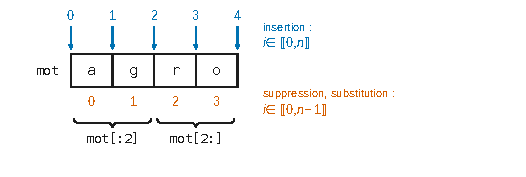
\includegraphics{figures/q1-indices-operations.pdf}
\caption*{Figure 1 --- Indices des opérations sur la chaîne `agro' (n = 4) : n + 1
positions d'insertion entre les caractères, n indices de caractère pour
la suppression et la substitution ; le préfixe `ag' et le suffixe `ro'
se séparent en position 2}
\end{figure}

\begin{piege}

Écrire \texttt{mot{[}:\allowbreak{}i{]}\allowbreak{}\ +\ c\ +\ mot{[}i+1:\allowbreak{}{]}\allowbreak{}} pour l'insertion redonne exactement \texttt{substitution}. Le code tourne sans erreur, d'où l'intérêt d'un contrôle par les longueurs : \(n-1\) pour une suppression, \(n\) pour une substitution, \(n+1\) pour une insertion.

\end{piege}

\begin{methode}

Les tranches Python ne lèvent jamais d'erreur, même hors bornes (\texttt{\textquotesingle{}agro\textquotesingle{}{[}10:{]}} vaut \texttt{\textquotesingle{}\textquotesingle{}}). Un indice faux donne un résultat silencieusement faux : vérifiez toujours une fonction de découpage sur un petit exemple, aux deux extrémités.

\end{methode}

\hypertarget{partie-ii-ruxe9solution-nauxefve-par-force-brute}{%
\section{Partie II --- Résolution naïve par force brute}\label{partie-ii-ruxe9solution-nauxefve-par-force-brute}}

On engendre toutes les chaînes à 1 opération de \texttt{mot1}, puis à 2, etc. La partie montre pourquoi cette idée simple est inutilisable : la taille des listes explose.

\hypertarget{question-2}{%
\subsection{Question 2}\label{question-2}}

\begin{indication}{1}

La liste \texttt{L} est construite au fur et à mesure : à quel moment faut-il ajouter \texttt{car}, et à quel moment faut-il s'abstenir ?

\end{indication}

\begin{indication}{2}

Le test d'appartenance \texttt{in} fonctionne sur une liste. Sur quelle liste doit-il porter ?

\end{indication}

\hypertarget{solution-2}{%
\subsubsection{Solution}\label{solution-2}}

\begin{lstlisting}[language=Python]
def lettres(mot):
    L = []
    for car in mot:
        if car not in L:       # ligne 4
            L.append(car)      # ligne 5
    return L
\end{lstlisting}

Invariant : avant chaque tour, \texttt{L} contient, sans répétition et dans l'ordre de première apparition, les caractères déjà parcourus. Pour \texttt{\textquotesingle{}concours\textquotesingle{}}, les caractères \texttt{c,\allowbreak{}\ o,\allowbreak{}\ n,\allowbreak{}\ c,\allowbreak{}\ o,\allowbreak{}\ u,\allowbreak{}\ r,\allowbreak{}\ s} sont lus, les seconds \texttt{c} et \texttt{o} sont écartés, d'où \texttt{{[}\textquotesingle{}c\textquotesingle{},\allowbreak{}\textquotesingle{}o\textquotesingle{},\allowbreak{}\textquotesingle{}n\textquotesingle{},\allowbreak{}\textquotesingle{}u\textquotesingle{},\allowbreak{}\textquotesingle{}r\textquotesingle{},\allowbreak{}\textquotesingle{}s\textquotesingle{}{]}\allowbreak{}}, conforme à l'énoncé.

\begin{piege}

Écrire \texttt{if\ car\ not\ in\ mot} : chaque caractère lu appartient évidemment à \texttt{mot}, le test est toujours faux, et la fonction renvoie la liste vide. Le test porte sur la liste en construction \texttt{L}.

\end{piege}

\hypertarget{question-3}{%
\subsection{Question 3}\label{question-3}}

\begin{indication}{1}

Lisez d'abord l'indentation : quels \texttt{append} sont dans la boucle sur \texttt{car}, lesquels n'y sont pas, et lesquels sont dans la boucle sur \texttt{i} ?

\end{indication}

\begin{indication}{2}

La boucle sur \texttt{i} ne parcourt que \(0,\dots,m-1\) où \(m\) est la longueur de \texttt{mot}. Combien de positions d'insertion y a-t-il, et laquelle n'est pas couverte par cette boucle ?

\end{indication}

\begin{indication}{3}

Un \texttt{append} sans variable \texttt{car} disponible ne peut correspondre qu'à une opération qui n'utilise aucun caractère.

\end{indication}

\hypertarget{solution-3}{%
\subsubsection{Solution}\label{solution-3}}

\begin{itemize}
\tightlist
\item
  Ligne 10 : dans la boucle sur \texttt{i}, hors de la boucle sur \texttt{car} : c'est la suppression à l'indice \texttt{i}.
\item
  Lignes 12 et 13 : dans la boucle sur \texttt{car} : substitution et insertion à l'indice \texttt{i} par le caractère \texttt{car}.
\item
  Ligne 15 : dans une boucle sur \texttt{car} placée \textbf{hors} de la boucle sur \texttt{i} : c'est l'insertion à la position \(m\), que la boucle sur \texttt{i} ne couvre pas.
\end{itemize}

\begin{lstlisting}[language=Python]
def force_brute(mot1, mot2):
    Dict = {0: [mot1]}
    d = 0
    lettres_mot2 = lettres(mot2)
    while True:
        d += 1
        Dict[d] = []
        for mot in Dict[d-1]:
            for i in range(len(mot)):
                Dict[d].append(suppression(mot, i))                 # ligne 10
                for car in lettres_mot2:
                    Dict[d].append(substitution(mot, i, car))       # ligne 12
                    Dict[d].append(insertion(mot, i, car))          # ligne 13
            for car in lettres_mot2:
                Dict[d].append(insertion(mot, len(mot), car))       # ligne 15
        if mot2 in Dict[d]:
            return d
\end{lstlisting}

Les lignes 12 et 13 peuvent être échangées. Pourquoi l'algorithme renvoie la distance : \texttt{Dict{[}d{]}} contient toutes les chaînes obtenues de \texttt{mot1} par \(d\) opérations dont les caractères insérés ou substitués sont des lettres de \texttt{mot2}. Une suite minimale de \texttt{mot1} à \texttt{mot2} peut toujours être choisie de cette façon (un caractère inséré ou substitué qui n'est pas dans \texttt{mot2} devrait être à nouveau modifié, ce qui ne serait pas minimal), donc \texttt{mot2} est dans \texttt{Dict{[}d{]}} pour \(d\) égal à la distance ; et toute chaîne de \texttt{Dict{[}d{]}} est à distance au plus \(d\) de \texttt{mot1}, donc \texttt{mot2} n'apparaît dans aucune vague antérieure.

\begin{piege}

Mettre \texttt{insertion(\allowbreak{}mot,\allowbreak{}\ i,\allowbreak{}\ car)\allowbreak{}} en ligne 15 : après la boucle, \texttt{i} vaut \(m-1\) et l'on n'insère jamais en fin de chaîne. Le programme ne plante pas (sauf si \texttt{mot1} est vide : \texttt{i} n'existe pas), mais il peut renvoyer une distance trop grande : de \texttt{\textquotesingle{}A\textquotesingle{}} à \texttt{\textquotesingle{}AB\textquotesingle{}}, il renvoie 2 au lieu de 1.

\end{piege}

\hypertarget{question-4-a}{%
\subsection{Question 4 a)}\label{question-4-a}}

\begin{indication}{1}

Commencez par calculer \texttt{lettres(\textquotesingle{}AGCTT\textquotesingle{})} : combien de caractères distincts ?

\end{indication}

\begin{indication}{2}

Comptez les \texttt{append} exécutés pour un mot de longueur \(m\), ligne par ligne, en fonction de \(m\) et du nombre \(k\) de caractères distincts de \texttt{mot2}.

\end{indication}

\begin{indication}{3}

La question porte sur le nombre d'éléments de la \textbf{liste} : un \texttt{append} ajoute toujours, même si la chaîne est déjà présente.

\end{indication}

\hypertarget{solution-4}{%
\subsubsection{Solution}\label{solution-4}}

\texttt{lettres(\allowbreak{}\textquotesingle{}AGCTT\textquotesingle{})\allowbreak{}\ =\allowbreak{}\ {[}\textquotesingle{}A\textquotesingle{},\allowbreak{}\textquotesingle{}G\textquotesingle{},\allowbreak{}\textquotesingle{}C\textquotesingle{},\allowbreak{}\textquotesingle{}T\textquotesingle{}{]}\allowbreak{}}, donc \(k=4\) (le \texttt{T} doublé n'est compté qu'une fois). Pour un mot de longueur \(m\) :

\begin{longtable}[]{@{}llll@{}}
\toprule\noalign{}
ligne & opération & nombre d'\texttt{append} & longueur produite \\
\midrule\noalign{}
\endhead
\bottomrule\noalign{}
\endlastfoot
10 & suppression & \(m\) & \(m-1\) \\
12 & substitution & \(km\) & \(m\) \\
13 & insertion aux indices \(0..m-1\) & \(km\) & \(m+1\) \\
15 & insertion en fin & \(k\) & \(m+1\) \\
\end{longtable}

Un mot de longueur \(m\) fournit donc \(N(m)\) éléments :

\equationajustee{\begin{aligned}
N(m) &= m+2km+k\\
&= (2k+1)m+k\\
&= 9m+4.
\end{aligned}}

\texttt{Dict{[}0{]}\allowbreak{}\ =\allowbreak{}\ {[}\textquotesingle{}ACG\textquotesingle{}{]}\allowbreak{}}, de longueur 3 :

\equationajustee{\begin{aligned}
|\texttt{Dict[1]}| &= N(3)\\
&= 9\times 3+4
\end{aligned}}

\equationajustee{\boxed{|\texttt{Dict[1]}| = 31}}

Ces 31 éléments ne sont pas tous distincts : \texttt{\textquotesingle{}ACG\textquotesingle{}} apparaît par exemple trois fois (substitution de chaque caractère par lui-même). Il n'y a que 26 chaînes distinctes, mais la question porte sur la liste.

\begin{piege}

Prendre \(k=5\) (la longueur de \texttt{mot2}) au lieu du nombre de caractères \textbf{distincts}, ou oublier les \(k\) insertions de la ligne 15 : on obtient 38 ou 27.

\end{piege}

\hypertarget{question-4-b}{%
\subsection{Question 4 b)}\label{question-4-b}}

\begin{indication}{1}

Le tableau précédent donne directement la longueur produite par chaque ligne du code.

\end{indication}

\hypertarget{solution-5}{%
\subsubsection{Solution}\label{solution-5}}

Avec \(m=3\) et \(k=4\) :

\begin{itemize}
\tightlist
\item
  les suppressions donnent \(m=3\) chaînes de longueur 2 ;
\item
  les substitutions donnent \(km=12\) chaînes de longueur 3 ;
\item
  les insertions (lignes 13 et 15) donnent \(k(m+1)=16\) chaînes de longueur 4.
\end{itemize}

\textbf{3 éléments de longueur 2, 12 de longueur 3, 16 de longueur 4} ; on retrouve bien \(3+12+16=31\).

\hypertarget{question-4-c}{%
\subsection{Question 4 c)}\label{question-4-c}}

\begin{indication}{1}

La boucle \texttt{while} s'arrête-t-elle après la première vague ? Regardez la longueur de \texttt{mot2}.

\end{indication}

\begin{indication}{2}

Chaque élément de \texttt{Dict{[}1{]}} est traité comme \texttt{mot1} l'a été, mais le nombre d'éléments qu'il fournit dépend de \textbf{sa} longueur.

\end{indication}

\hypertarget{solution-6}{%
\subsubsection{Solution}\label{solution-6}}

\texttt{mot2\ =\ \textquotesingle{}AGCTT\textquotesingle{}} est de longueur 5 alors que \texttt{Dict{[}1{]}} ne contient que des chaînes de longueurs 2 à 4 : le test de la ligne 16 échoue et \texttt{Dict{[}2{]}} est construit. Chacun des 31 éléments de \texttt{Dict{[}1{]}} (doublons compris) fournit \(N(m)\) éléments. On a \(N(2)=22\), \(N(3)=31\) et \(N(4)=40\) :

\equationajustee{\begin{aligned}
|\texttt{Dict[2]}| &= 3\times 22+12\times 31+16\times 40\\
&= 66+372+640
\end{aligned}}

\equationajustee{\boxed{|\texttt{Dict[2]}| = 1078}}

Contrôle : la somme des longueurs des 31 éléments vaut \(6+36+64=106\), donc

\equationajustee{\begin{aligned}
|\texttt{Dict[2]}| &= 9\times 106+4\times 31\\
&= 954+124\\
&= 1078.
\end{aligned}}

\begin{methode}

Pour compter ce que produit un programme, comptez les instructions exécutées en fonction des paramètres (ici \(m\) et \(k\)), puis sommez en regroupant les entrées par paramètre : c'est exactement le rôle de la question b). En poursuivant ainsi, on trouve \(42\,562\) éléments dans \texttt{Dict{[}3{]}}, vague où \texttt{\textquotesingle{}AGCTT\textquotesingle{}} apparaît enfin (la distance vaut 3) : la croissance est exponentielle en \(d\).

\end{methode}

\begin{piege}

Écrire \(|\texttt{Dict[2]}|=31\times 31=961\), comme si tous les éléments de \texttt{Dict{[}1{]}} avaient la longueur de \texttt{mot1}.

\end{piege}

\hypertarget{partie-iii-ruxe9solution-par-programmation-dynamique}{%
\section{Partie III --- Résolution par programmation dynamique}\label{partie-iii-ruxe9solution-par-programmation-dynamique}}

La relation de récurrence est donnée : \(D(i,j)\) ne dépend que des trois cases voisines au-dessus, à gauche et en diagonale. Il suffit de remplir le tableau dans un ordre où ces cases sont toujours déjà calculées.

\hypertarget{question-5}{%
\subsection{Question 5}\label{question-5}}

\begin{indication}{1}

Écrivez les caractères de \texttt{mot2} au-dessus des colonnes et ceux de \texttt{mot1} à gauche des lignes, décalés d'une case comme dans l'exemple : la case \((i,j)\) compare le caractère de la ligne \(i\) et celui de la colonne \(j\).

\end{indication}

\begin{indication}{2}

Repérez d'abord les cases où les caractères sont égaux : elles recopient la case diagonale \textbf{sans} ajouter 1. Les autres valent 1 plus le minimum des trois voisines.

\end{indication}

\hypertarget{solution-7}{%
\subsubsection{Solution}\label{solution-7}}

\begin{figure}[H]
\centering
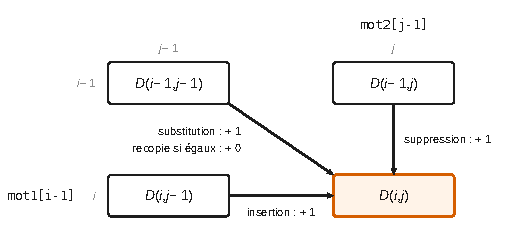
\includegraphics{figures/q5-dependances-case.pdf}
\caption*{Figure 2 --- Les trois cases dont dépend D(i, j) : insertion depuis la
gauche, suppression depuis le haut, substitution depuis la diagonale,
chacune de coût 1 ; recopie gratuite de la diagonale si les deux
caractères comparés sont égaux}
\end{figure}

\texttt{mot1\ =\ \textquotesingle{}ACTCT\textquotesingle{}} indexe les lignes, \texttt{mot2\ =\ \textquotesingle{}AGTCAG\textquotesingle{}} les colonnes. Les cases d'égalité sont :

\begin{itemize}
\tightlist
\item
  \texttt{A} : cases (1,1) et (1,5) ;
\item
  \texttt{C} : cases (2,4) et (4,4) ;
\item
  \texttt{T} : cases (3,3) et (5,3).
\end{itemize}

Détail de quelques cases (dans le cas général, les trois nombres du minimum sont, dans l'ordre, les voisines gauche, haut et diagonale) :

\begin{longtable}[]{@{}llll@{}}
\toprule\noalign{}
case & caractères & calcul & valeur \\
\midrule\noalign{}
\endhead
\bottomrule\noalign{}
\endlastfoot
(1,1) & \texttt{A} = \texttt{A} & \(D(0,0)\) & 0 \\
(1,2) & \texttt{A} ≠ \texttt{G} & \(1+\min(0,2,1)\) & 1 \\
(1,5) & \texttt{A} = \texttt{A} & \(D(0,4)\) & 4 \\
(2,1) & \texttt{C} ≠ \texttt{A} & \(1+\min(2,0,1)\) & 1 \\
(2,4) & \texttt{C} = \texttt{C} & \(D(1,3)\) & 2 \\
(3,3) & \texttt{T} = \texttt{T} & \(D(2,2)\) & 1 \\
(3,4) & \texttt{T} ≠ \texttt{C} & \(1+\min(1,2,2)\) & 2 \\
(4,4) & \texttt{C} = \texttt{C} & \(D(3,3)\) & 1 \\
(4,5) & \texttt{C} ≠ \texttt{A} & \(1+\min(1,3,2)\) & 2 \\
(4,6) & \texttt{C} ≠ \texttt{G} & \(1+\min(2,4,3)\) & 3 \\
(5,3) & \texttt{T} = \texttt{T} & \(D(4,2)\) & 3 \\
(5,5) & \texttt{T} ≠ \texttt{A} & \(1+\min(2,2,1)\) & 2 \\
(5,6) & \texttt{T} ≠ \texttt{G} & \(1+\min(2,3,2)\) & 3 \\
\end{longtable}

\begin{longtable}[]{@{}llllllll@{}}
\toprule\noalign{}
& & A & G & T & C & A & G \\
\midrule\noalign{}
\endhead
\bottomrule\noalign{}
\endlastfoot
& \textbf{0} & 1 & 2 & 3 & 4 & 5 & 6 \\
\textbf{A} & 1 & 0 & 1 & 2 & 3 & 4 & 5 \\
\textbf{C} & 2 & 1 & 1 & 2 & 2 & 3 & 4 \\
\textbf{T} & 3 & 2 & 2 & 1 & 2 & 3 & 4 \\
\textbf{C} & 4 & 3 & 3 & 2 & 1 & 2 & 3 \\
\textbf{T} & 5 & 4 & 4 & 3 & 2 & 2 & \textbf{3} \\
\end{longtable}

\equationajustee{\boxed{D(5,6)=3}}

\begin{methode}

Deux contrôles gratuits : deux cases voisines (horizontalement, verticalement ou en diagonale descendante) diffèrent d'au plus 1, et \(|i-j|\le D(i,j)\le\max(i,j)\). Ici \(1\le 3\le 6\).

\end{methode}

\begin{piege}

Ajouter 1 dans le cas d'égalité : le tableau n'a plus aucun « creux » diagonal et l'on trouve \(D(5,6)=6\).

\end{piege}

\hypertarget{question-6}{%
\subsection{Question 6}\label{question-6}}

\begin{indication}{1}

Deux critères : les dimensions (\(n+1\) lignes de \(p+1\) éléments) et l'indépendance des lignes, puisqu'on va modifier les cases une par une.

\end{indication}

\begin{indication}{2}

Que se passe-t-il en mémoire lorsqu'on multiplie par un entier une liste dont l'élément est lui-même une liste ?

\end{indication}

\hypertarget{solution-8}{%
\subsubsection{Solution}\label{solution-8}}

\textbf{\texttt{matrice\_nulle\_1} et \texttt{matrice\_nulle\_4}.}

Justification (non demandée) :

\begin{itemize}
\tightlist
\item
  \texttt{matrice\_nulle\_1} : l'expression \texttt{{[}0{]}*(p+1)} est réévaluée à chaque tour de la compréhension : \(n+1\) listes distinctes de \(p+1\) zéros. Convient.
\item
  \texttt{matrice\_nulle\_2} : \texttt{{[}0{]}*(p+1)} est évaluée une seule fois, et \texttt{*\ (n+1)} recopie \(n+1\) fois la \textbf{référence} à cette même liste. Après \texttt{M{[}0{]}{[}0{]}\ =\ 7}, toute la colonne 0 vaut 7. Ne convient pas.
\item
  \texttt{matrice\_nulle\_3} : \(p+1\) lignes de \(n+1\) éléments, c'est la transposée ; dès que \(n\neq p\), l'accès \texttt{D{[}n{]}{[}p{]}} sort des bornes. Ne convient pas.
\item
  \texttt{matrice\_nulle\_4} : \(n+1\) lignes indépendantes (une nouvelle liste \texttt{L} à chaque tour) de \(p+1\) zéros. Convient.
\end{itemize}

\begin{figure}[H]
\centering
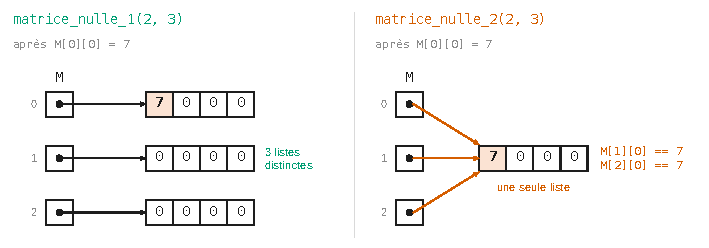
\includegraphics{figures/q6-alias-matrice-nulle.pdf}
\caption*{Figure 3 --- Listes en mémoire pour n = 2 et p = 3, après avoir mis 7
dans la case (0, 0) : matrice\_nulle\_1 crée trois listes distinctes,
matrice\_nulle\_2 trois références vers une même liste, dont toute la
colonne 0 vaut alors 7}
\end{figure}

\begin{piege}

\texttt{{[}0{]}*(p+1)} est sans danger car l'entier 0 n'est pas modifiable ; c'est la répétition d'un objet \textbf{modifiable} (une liste) qui crée des alias. Pour s'en convaincre, simuler \texttt{M{[}0{]}{[}0{]}\ =\ 1} sur une matrice \(2\times 2\).

\end{piege}

\hypertarget{question-7}{%
\subsection{Question 7}\label{question-7}}

\begin{indication}{1}

Chaque ligne à compléter correspond à une ligne de la relation de récurrence encadrée de l'énoncé, dans l'ordre : création du tableau, bord \(i=0\), bord \(j=0\), cas d'égalité, cas général.

\end{indication}

\begin{indication}{2}

Pour la ligne 3, utilisez la fonction de la question 6 avec les arguments dans le bon ordre (lignes d'abord).

\end{indication}

\hypertarget{solution-9}{%
\subsubsection{Solution}\label{solution-9}}

\begin{lstlisting}[language=Python]
def matrice_levenshtein(mot1, mot2):
    n, p = len(mot1), len(mot2)
    D = matrice_nulle(n, p)                                         # ligne 3
    for j in range(p+1):
        D[0][j] = j                                                 # ligne 5
    for i in range(n+1):
        D[i][0] = i                                                 # ligne 7
    for i in range(1, n+1):
        for j in range(1, p+1):
            if mot1[i-1] == mot2[j-1]:
                D[i][j] = D[i-1][j-1]                               # ligne 11
            else:
                D[i][j] = 1 + min(D[i][j-1], D[i-1][j], D[i-1][j-1])  # ligne 13
    return D
\end{lstlisting}

Le parcours par lignes croissantes puis colonnes croissantes garantit que les trois cases voisines (gauche, haut, diagonale) sont déjà remplies quand on calcule la case \((i,j)\). La fonction effectue \(np\) tours de la double boucle : temps et mémoire en \(O(np)\), à comparer à la croissance exponentielle de \texttt{force\_brute}.

\begin{piege}

Mettre le \texttt{+1} à l'intérieur d'un seul terme du minimum, ou oublier le terme diagonal \(D(i-1,j-1)\) (on interdirait alors les substitutions).

\end{piege}

\begin{jury}

Dans un texte à trous, on recopie le squelette avec ses numéros de ligne et l'on complète exactement les lignes demandées, sans réorganiser le code ni renommer les variables.

\end{jury}

\hypertarget{question-8}{%
\subsection{Question 8}\label{question-8}}

\begin{indication}{1}

L'énoncé dit quelle case de la matrice contient la distance d'édition de \texttt{mot1} à \texttt{mot2}.

\end{indication}

\hypertarget{solution-10}{%
\subsubsection{Solution}\label{solution-10}}

La distance cherchée est \(D(n,p)\), case en bas à droite :

\begin{lstlisting}[language=Python]
def distance(mot1, mot2):
    D = matrice_levenshtein(mot1, mot2)
    return D[len(mot1)][len(mot2)]
\end{lstlisting}

(\texttt{return\ D{[}-1{]}{[}-1{]}} est équivalent.) Sur les exemples : \texttt{distance(\allowbreak{}\textquotesingle{}ACT\textquotesingle{},\allowbreak{}\textquotesingle{}AGTC\textquotesingle{})\allowbreak{}} vaut 2, \texttt{distance(\allowbreak{}\textquotesingle{}ACTCT\textquotesingle{},\allowbreak{}\textquotesingle{}AGTCAG\textquotesingle{})\allowbreak{}} vaut 3, et \texttt{distance(\allowbreak{}\textquotesingle{}CAGTA\textquotesingle{},\allowbreak{}\textquotesingle{}AGGTC\textquotesingle{})\allowbreak{}} vaut 3, ce qui confirme la valeur annoncée dans l'introduction.

\begin{piege}

Écrire \texttt{D{[}len(\allowbreak{}mot2)\allowbreak{}{]}\allowbreak{}{[}len(\allowbreak{}mot1)\allowbreak{}{]}\allowbreak{}} : les lignes sont indexées par \texttt{mot1}. Avec \texttt{\textquotesingle{}ACTCT\textquotesingle{}} et \texttt{\textquotesingle{}AGTCAG\textquotesingle{}}, cela lit \texttt{D{[}6{]}}, qui n'existe pas.

\end{piege}

\hypertarget{partie-iv-application-correcteur-orthographique}{%
\section{Partie IV --- Application : correcteur orthographique}\label{partie-iv-application-correcteur-orthographique}}

On parcourt une seule fois le dictionnaire en tenant à jour à la fois la meilleure distance et la liste des mots qui la réalisent.

\hypertarget{question-9}{%
\subsection{Question 9}\label{question-9}}

\begin{indication}{1}

Ligne 6 : quelle fonction déjà écrite renvoie un \textbf{entier} comparable à \texttt{dmin} ?

\end{indication}

\begin{indication}{2}

Lorsqu'on trouve un mot strictement plus proche que tous les précédents, que deviennent les mots déjà retenus dans \texttt{M} ? Et en cas d'égalité ?

\end{indication}

\hypertarget{solution-11}{%
\subsubsection{Solution}\label{solution-11}}

\begin{lstlisting}[language=Python]
def correcteur_orthographique(mot):
    n = len(mot)
    dmin = n+1
    M = []
    for chaine in Mots_Francais:
        d = distance(mot, chaine)       # ligne 6
        if d < dmin:
            dmin = d
            M = [chaine]                # ligne 9
        elif d == dmin:
            M.append(chaine)            # ligne 11
    return M
\end{lstlisting}

Invariant : après chaque tour, \texttt{dmin} est la plus petite distance de \texttt{mot} aux mots déjà examinés et \texttt{M} la liste de ces mots qui la réalisent. Un nouveau record invalide tous les mots précédents (ligne 9 : on repart d'une liste réduite à \texttt{chaine}) ; une égalité ajoute \texttt{chaine} (ligne 11). L'initialisation \texttt{dmin\ =\ n+1} est sûre : le mot \texttt{\textquotesingle{}a\textquotesingle{}} est à distance au plus \(\max(n,1)\le n+1\) de \texttt{mot}, donc au moins un mot est retenu.

Pour \texttt{\textquotesingle{}mason\textquotesingle{}}, \texttt{\textquotesingle{}macon\textquotesingle{}}, \texttt{\textquotesingle{}maçon\textquotesingle{}}, \texttt{\textquotesingle{}maton\textquotesingle{}} sont à distance 1 (une substitution), \texttt{\textquotesingle{}maison\textquotesingle{}} aussi (une insertion), et aucun mot n'est à distance 0 : on obtient bien \texttt{{[}\textquotesingle{}macon\textquotesingle{},\allowbreak{}\textquotesingle{}maçon\textquotesingle{},\allowbreak{}\textquotesingle{}maison\textquotesingle{},\allowbreak{}\textquotesingle{}maton\textquotesingle{}{]}\allowbreak{}}, dans l'ordre du dictionnaire.

\begin{piege}

Écrire \texttt{M.append(chaine)} en ligne 9 : la liste contiendrait tous les records successifs (\texttt{\textquotesingle{}a\textquotesingle{}}, à distance 4, en tête). Autre erreur : remplacer \texttt{elif} par un second \texttt{if}, ce qui ajoute deux fois le mot qui vient d'établir le record.

\end{piege}

\begin{methode}

Le schéma « minimum et liste des éléments qui le réalisent » en un seul parcours est très classique : réinitialiser la liste sur une amélioration stricte, la compléter sur une égalité.

\end{methode}

\hypertarget{partie-v-obtention-dune-suite-dopuxe9rations-minimale}{%
\section{Partie V --- Obtention d'une suite d'opérations minimale}\label{partie-v-obtention-dune-suite-dopuxe9rations-minimale}}

On lit la matrice à l'envers, de \((n,p)\) vers \((0,0)\), en transformant progressivement \texttt{mot2} en \texttt{mot1}. Un bon fil conducteur est la chaîne associée à la case \((i,j)\) :

\equationajustee{\texttt{mot}(i,j)=\texttt{mot2[:j]}+\texttt{mot1[i:]}}

Son début est déjà conforme à la cible, sa fin est encore celle de la source. Le jury considérait cette partie comme largement hors barème (voir l'encadré de Q 10).

\hypertarget{question-10}{%
\subsection{Question 10}\label{question-10}}

\begin{indication}{1}

Appliquez les règles de l'énoncé case par case, en partant de \((5,6)\) ; lorsque les caractères diffèrent, testez \textbf{les trois} provenances, chacune pouvant ouvrir une branche.

\end{indication}

\begin{indication}{2}

Quand les caractères sont égaux, l'énoncé impose la remontée en diagonale sans opération : pas de branche à ouvrir.

\end{indication}

\begin{indication}{3}

Pour contrôler chaque chaîne intermédiaire, vérifiez qu'elle commence par les \(j\) premiers caractères de \texttt{mot2} et finit par les caractères de \texttt{mot1} à partir de l'indice \(i\).

\end{indication}

\hypertarget{solution-12}{%
\subsubsection{Solution}\label{solution-12}}

On utilise la matrice de la question 5. Le tableau donne, pour chaque case visitée, la valeur des trois voisines ; une voisine est retenue (« oui ») si elle vaut \(D(i,j)-1\). Aux cases d'égalité, la méthode impose la diagonale sans opération.

\begin{longtable}[]{@{}
  >{\raggedright\arraybackslash}p{(\columnwidth - 14\tabcolsep) * \real{0.0886}}
  >{\raggedright\arraybackslash}p{(\columnwidth - 14\tabcolsep) * \real{0.0687}}
  >{\raggedright\arraybackslash}p{(\columnwidth - 14\tabcolsep) * \real{0.1535}}
  >{\raggedright\arraybackslash}p{(\columnwidth - 14\tabcolsep) * \real{0.1254}}
  >{\raggedright\arraybackslash}p{(\columnwidth - 14\tabcolsep) * \real{0.1189}}
  >{\raggedright\arraybackslash}p{(\columnwidth - 14\tabcolsep) * \real{0.0971}}
  >{\raggedright\arraybackslash}p{(\columnwidth - 14\tabcolsep) * \real{0.0971}}
  >{\raggedright\arraybackslash}p{(\columnwidth - 14\tabcolsep) * \real{0.2207}}@{}}
\toprule\noalign{}
\begin{minipage}[b]{\linewidth}\raggedright
case
\end{minipage} & \begin{minipage}[b]{\linewidth}\raggedright
\(D\)
\end{minipage} & \begin{minipage}[b]{\linewidth}\raggedright
chaîne courante
\end{minipage} & \begin{minipage}[b]{\linewidth}\raggedright
caractères
\end{minipage} & \begin{minipage}[b]{\linewidth}\raggedright
diagonale
\end{minipage} & \begin{minipage}[b]{\linewidth}\raggedright
gauche
\end{minipage} & \begin{minipage}[b]{\linewidth}\raggedright
haut
\end{minipage} & \begin{minipage}[b]{\linewidth}\raggedright
pas effectué
\end{minipage} \\
\midrule\noalign{}
\endhead
\bottomrule\noalign{}
\endlastfoot
(5,6) & 3 & \texttt{AGTCAG} & \texttt{T} ≠ \texttt{G} & 2, oui & 2, oui & 3, non & deux branches \\
(4,5) & 2 & \texttt{AGTCAT} & \texttt{C} ≠ \texttt{A} & 2, non & 1, oui & 3, non & suppression de l'indice 4 \\
(5,5) & 2 & \texttt{AGTCA} & \texttt{T} ≠ \texttt{A} & 1, oui & 2, non & 2, non & substitution de l'indice 4 par \texttt{T} \\
(4,4) & 1 & \texttt{AGTCT} & \texttt{C} = \texttt{C} & & & & diagonale, sans opération \\
(3,3) & 1 & \texttt{AGTCT} & \texttt{T} = \texttt{T} & & & & diagonale, sans opération \\
(2,2) & 1 & \texttt{AGTCT} & \texttt{C} ≠ \texttt{G} & 0, oui & 1, non & 1, non & substitution de l'indice 1 par \texttt{C} \\
(1,1) & 0 & \texttt{ACTCT} & \texttt{A} = \texttt{A} & & & & diagonale vers (0,0) \\
\end{longtable}

\begin{itemize}
\tightlist
\item
  \textbf{Branche 1}, par (4,5) : en (5,6), substitution à l'indice \(j-1=5\) par \texttt{mot1{[}4{]}\ =\ \textquotesingle{}T\textquotesingle{}}, d'où \texttt{AGTCAT} ; puis suppression de l'indice 4, d'où \texttt{AGTCT} en (4,4).
\item
  \textbf{Branche 2}, par (5,5) : en (5,6), suppression de l'indice 5, d'où \texttt{AGTCA} ; puis substitution de l'indice 4 par \texttt{mot1{[}4{]}\ =\ \textquotesingle{}T\textquotesingle{}}, d'où \texttt{AGTCT} en (4,4).
\item
  \textbf{Tronc commun} depuis (4,4) : deux diagonales sans opération jusqu'en (2,2) ; là, substitution de l'indice 1 par \texttt{mot1{[}1{]}\ =\ \textquotesingle{}C\textquotesingle{}}, d'où \texttt{ACTCT} en (1,1) ; enfin une diagonale vers (0,0).
\end{itemize}

Aucune autre bifurcation : il y a \textbf{exactement deux suites minimales}, de 3 opérations chacune :

\equationajustee{\boxed{\begin{aligned}{}&\texttt{ACTCT}\longrightarrow\texttt{AGTCT}\longrightarrow\texttt{AGTCAT}\longrightarrow\texttt{AGTCAG}\\
&\texttt{ACTCT}\longrightarrow\texttt{AGTCT}\longrightarrow\texttt{AGTCA}\longrightarrow\texttt{AGTCAG}
\end{aligned}}}

Dans le sens direct, la première substitue \texttt{C}→\texttt{G} (indice 1), insère \texttt{A} (indice 4) puis substitue \texttt{T}→\texttt{G} (indice 5) ; la seconde substitue \texttt{C}→\texttt{G} (indice 1), substitue \texttt{T}→\texttt{A} (indice 4) puis insère \texttt{G} (indice 5). Les chemins correspondants dans la matrice se séparent en \((4,4)\) : la branche 1 passe par \((4,5)\), la branche 2 par \((5,5)\).

\begin{figure}[H]
\centering
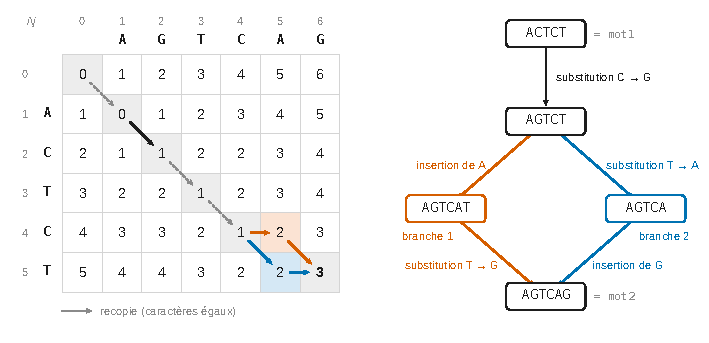
\includegraphics{figures/q10-chemins-matrice.pdf}
\caption*{Figure 4 --- Les deux chemins optimaux dans la matrice D de la question
5, orientés de (0,0) vers (5,6) (la remontée les parcourt à l'envers),
et les deux suites minimales de 3 opérations de ACTCT à AGTCAG}
\end{figure}

\begin{piege}

Les opérations lues pendant la remontée sont les \textbf{inverses} de celles de la suite : quand la remontée supprime un caractère, la suite lue de \texttt{mot1} vers \texttt{mot2} l'insère. Il faut présenter les suites de \texttt{mot1} vers \texttt{mot2}.

\end{piege}

\begin{methode}

Pour trouver \textbf{toutes} les solutions, faites l'arbre des choix : à chaque case, testez systématiquement les trois provenances et notez chaque bifurcation, puis vérifiez si les branches se rejoignent.

\end{methode}

\begin{jury}

Le rapport 2026 situe la partie V à part : « Cette dernière partie était estimée un peu hors-barème, destinée aux seuls candidats de niveau exceptionnel, s'il en est. » Il ne la commente pas davantage. En 45 minutes, Q 10 et Q 11 ne se traitent donc qu'après avoir sécurisé les parties I à IV ; une remontée bâclée rapporte peu.

\end{jury}

\hypertarget{question-11}{%
\subsection{Question 11}\label{question-11}}

\begin{indication}{1}

Ligne 2 : les lignes 9, 13 et 17 lisent des cases de \texttt{D} ; il faut donc la matrice entière, pas seulement la distance.

\end{indication}

\begin{indication}{2}

Les lignes 10, 14 et 18 traduisent mot pour mot les trois règles de la partie V, avec les fonctions de la partie I. Relisez à quel indice et avec quel caractère chaque opération se fait.

\end{indication}

\begin{indication}{3}

Les indices dans la chaîne courante sont donnés par \(j\) (position dans la cible déjà construite) ; le caractère utilisé vient de \texttt{mot1}.

\end{indication}

\hypertarget{solution-13}{%
\subsubsection{Solution}\label{solution-13}}

\begin{lstlisting}[language=Python]
def suite_operations(mot1, mot2):
    D = matrice_levenshtein(mot1, mot2)                 # ligne 2
    Suite_chgt = [mot2]
    mot = mot2
    i, j = len(mot1), len(mot2)
    while i > 0 or j > 0:
        if i>0 and j>0 and mot1[i-1] == mot2[j-1]:
            i, j = i-1, j-1
        elif i>0 and j>0 and D[i-1][j-1] == D[i][j]-1:
            mot = substitution(mot, j-1, mot1[i-1])     # ligne 10
            i, j = i-1, j-1
            Suite_chgt = [mot] + Suite_chgt
        elif j > 0 and D[i][j-1] == D[i][j] -1:
            mot = suppression(mot, j-1)                 # ligne 14
            j = j-1
            Suite_chgt = [mot] + Suite_chgt
        elif i > 0 and D[i-1][j] == D[i][j]-1:
            mot = insertion(mot, j, mot1[i-1])          # ligne 18
            Suite_chgt = [mot] + Suite_chgt
            i = i-1
    return Suite_chgt
\end{lstlisting}

Justification par l'invariant \(\texttt{mot}=\texttt{mot2[:j]}+\texttt{mot1[i:]}\), vrai au départ (\(\texttt{mot2}+\texttt{''}\)) :

\begin{itemize}
\tightlist
\item
  substitution vers \((i-1,j-1)\) : on remplace le caractère d'indice \(j-1\) (qui est \texttt{mot2{[}j-1{]}}) par \texttt{mot1{[}i-1{]}}, et l'on obtient \(\texttt{mot2[:j-1]}+\texttt{mot1[i-1:]}\) ;
\item
  suppression vers \((i,j-1)\) : on retire le caractère d'indice \(j-1\), d'où \(\texttt{mot2[:j-1]}+\texttt{mot1[i:]}\) ;
\item
  insertion vers \((i-1,j)\) : on insère \texttt{mot1{[}i-1{]}} à l'indice \(j\), juste après \texttt{mot2{[}:j{]}}, d'où \(\texttt{mot2[:j]}+\texttt{mot1[i-1:]}\) ;
\item
  cas d'égalité : \(\texttt{mot2[:j-1]}+\texttt{mot1[i-1:]}\) est la même chaîne, rien à faire.
\end{itemize}

En (0,0), \texttt{mot} vaut donc \texttt{mot1}. La boucle termine, car \(i+j\) décroît strictement.

Elle ne se bloque jamais : hors des bords, la relation de récurrence garantit qu'une voisine vaut \(D(i,j)-1\) ; sur les bords, les valeurs initiales \(D(0,j)=j\) et \(D(i,0)=i\) le garantissent aussi.

La liste renvoyée contient \(D(n,p)+1\) chaînes : la suite est minimale. Sur l'exemple de Q 10, la diagonale étant testée avant la gauche, la fonction renvoie \texttt{{[}\textquotesingle{}ACTCT\textquotesingle{},\allowbreak{}\ \textquotesingle{}AGTCT\textquotesingle{},\allowbreak{}\ \textquotesingle{}AGTCAT\textquotesingle{},\allowbreak{}\ \textquotesingle{}AGTCAG\textquotesingle{}{]}\allowbreak{}}.

\begin{piege}

Écrire \texttt{substitution(\allowbreak{}mot,\allowbreak{}\ i-1,\allowbreak{}\ mot1{[}i-1{]}\allowbreak{})\allowbreak{}} : c'est juste tant que \(i=j\), faux dès que le chemin quitte la diagonale principale. Autre confusion : insérer à l'indice \(j-1\) au lieu de \(j\).

\end{piege}

\begin{methode}

Pour compléter un code de reconstruction, écrivez l'invariant qui relie la variable courante aux indices de boucle et vérifiez qu'il est préservé par chaque branche : il donne les indices sans hésitation.

\end{methode}

\hypertarget{bilan}{%
\section{Bilan}\label{bilan}}

\textbf{Méthodes à retenir.}

\begin{itemize}
\tightlist
\item
  Manipuler des chaînes non modifiables par tranches et concaténation ; contrôler par les longueurs et sur les cas extrêmes (\(i=0\), \(i=n\)).
\item
  Lire l'indentation d'un squelette avant de compléter : elle dit quelles variables sont disponibles à chaque ligne.
\item
  Dénombrer les opérations d'un programme en fonction de ses paramètres, puis regrouper par paramètre (ici la longueur des mots).
\item
  Programmation dynamique : une récurrence sur des sous-problèmes (préfixes), un tableau, un ordre de remplissage qui rend disponibles les cases dont on a besoin, puis éventuellement une \textbf{remontée} dans le tableau pour reconstruire une solution optimale.
\item
  Schéma « minimum et tous ses réalisateurs » en un seul parcours.
\end{itemize}

\textbf{Prérequis à revoir.} Tranches et concaténation de chaînes ; test \texttt{in} ; listes de listes et piège de \texttt{{[}{[}0{]}*p{]}*n} ; dictionnaires indexés par des entiers ; boucles imbriquées et invariants.

\textbf{Leçons du rapport 2026.} Le sujet était volontairement trop long pour 45 minutes, avec 8 points sur 28 hors barème, et la partie V réservée aux meilleurs. Il faut donc d'abord rédiger juste et vite les parties I à IV, et contrôler chaque réponse sur un exemple plutôt que de répondre au jugé.

\textbf{Questions classiques transposables.} Initialisation correcte d'une matrice en Python (aliasing) ; remplissage d'un tableau de programmation dynamique (plus longue sous-séquence commune, rendu de monnaie, sac à dos) ; reconstruction d'une solution optimale à partir du tableau ; comparaison d'une méthode exhaustive exponentielle et d'une méthode en \(O(np)\).

\end{document}
